\section{Diagramma dei Casi d'Uso}

In questa sezione viene presentato il diagramma dei casi d'uso dell'applicazione sviluppata. In particolare, con riferimento a quanto descritto nella sezione introduttiva, l'applicativo deve essere in grado di fornire le funzionalità di base di una applicazione di messaggistica, tralasciando le ipotesi di sicurezza, valutate in fase di design. Per motivo, sono stati individuati tra casi d'uso:
\begin{itemize}
	\item Login, funzionalità che assolve all'autenticazione degli utenti;
	\item Registrazione, funzionalità che assolve all'iscrizione nel sistema degli utenti;
	\item Chat, funzionalità core del sistema.
\end{itemize}

Inoltre, rispettando il requisito di Two-Factor Authentication, si è preposto un relativo caso d'uso d'estensione, che si attiva quando all'atto del login, l'IP risulta essere sconosciuto.

Il risultato è mostrato in figura \ref{gfx:ucdiagram}.

\begin{figure}[!htbp]
	\centering
	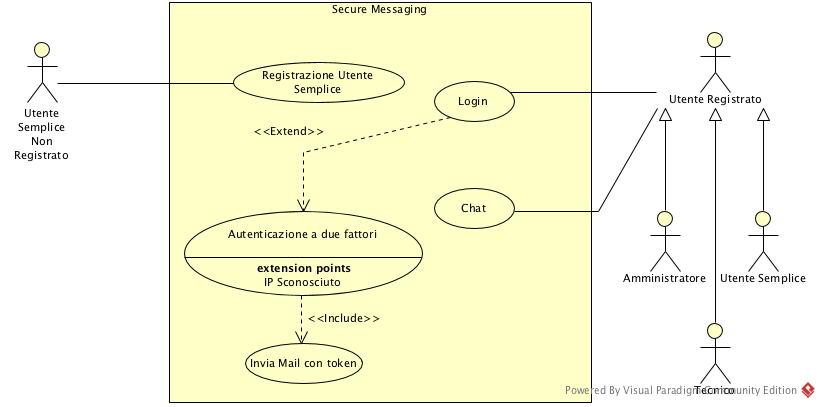
\includegraphics[scale = .4]{img/UseCase.jpg}
	\caption{Diagramma dei Casi d'Uso}
	\label{gfx:ucdiagram}
\end{figure}

In particolare, è da notarsi la gerarchia di utenti specificata, conforme a quanto specificato in fase di introduzione.